\documentclass[a4paper,12pt]{article}
\usepackage[utf8]{inputenc}
\usepackage{amsmath}
\usepackage{array}
\usepackage{amsfonts}
\usepackage{graphicx}
\usepackage{hyperref}
\usepackage{fancyhdr}
\usepackage{geometry}
\usepackage{indentfirst}
\usepackage{hhline}
\usepackage{ulem}
\usepackage{cite}
\usepackage{caption}
\geometry{margin=1in}

\setlength{\parindent}{15pt} % Set the ginbal paragraph indentation to 15pt
% \addtolength{\topmargin}{-2.5pt} % Adjust the top margin to compensate
\pagestyle{fancy} % Use the fancyhdr package

% Clear all header and footer fields
\fancyhf{}

% Define the header for the first page
\fancypagestyle{cover}{
  \fancyhf{} % Clear all header and footer fields
  \fancyhead[C]{
    \parbox{0.95\textwidth}{\centering
      \fontsize{12}{14}\selectfont BME 12 - Medical robotics, cyber physical engineering and virtual reality
    }
    \vspace{2pt}
  }
}

\pagestyle{plain}

\title{Robotic Finger Modeling Project}
\author{\textbf{Charalampos Inglezos}}

\begin{document}
\newgeometry{margin=1in, headheight=28pt}
% Title Page
\begin{titlepage}
    \thispagestyle{cover} % Apply the cover style to this page
    \centering
    \vspace*{4pt}
    \Large
    Aristotle University of Thessaloniki\\
    \Huge
    \textbf{Robotic Finger Modeling Project}\\
    \vspace{8pt}
    \LARGE\textbf{Personal Report}
    
    \vspace{1cm}
    
    \LARGE
    \textbf{Charalampos Inglezos}
    
    \vspace{2cm}
    
    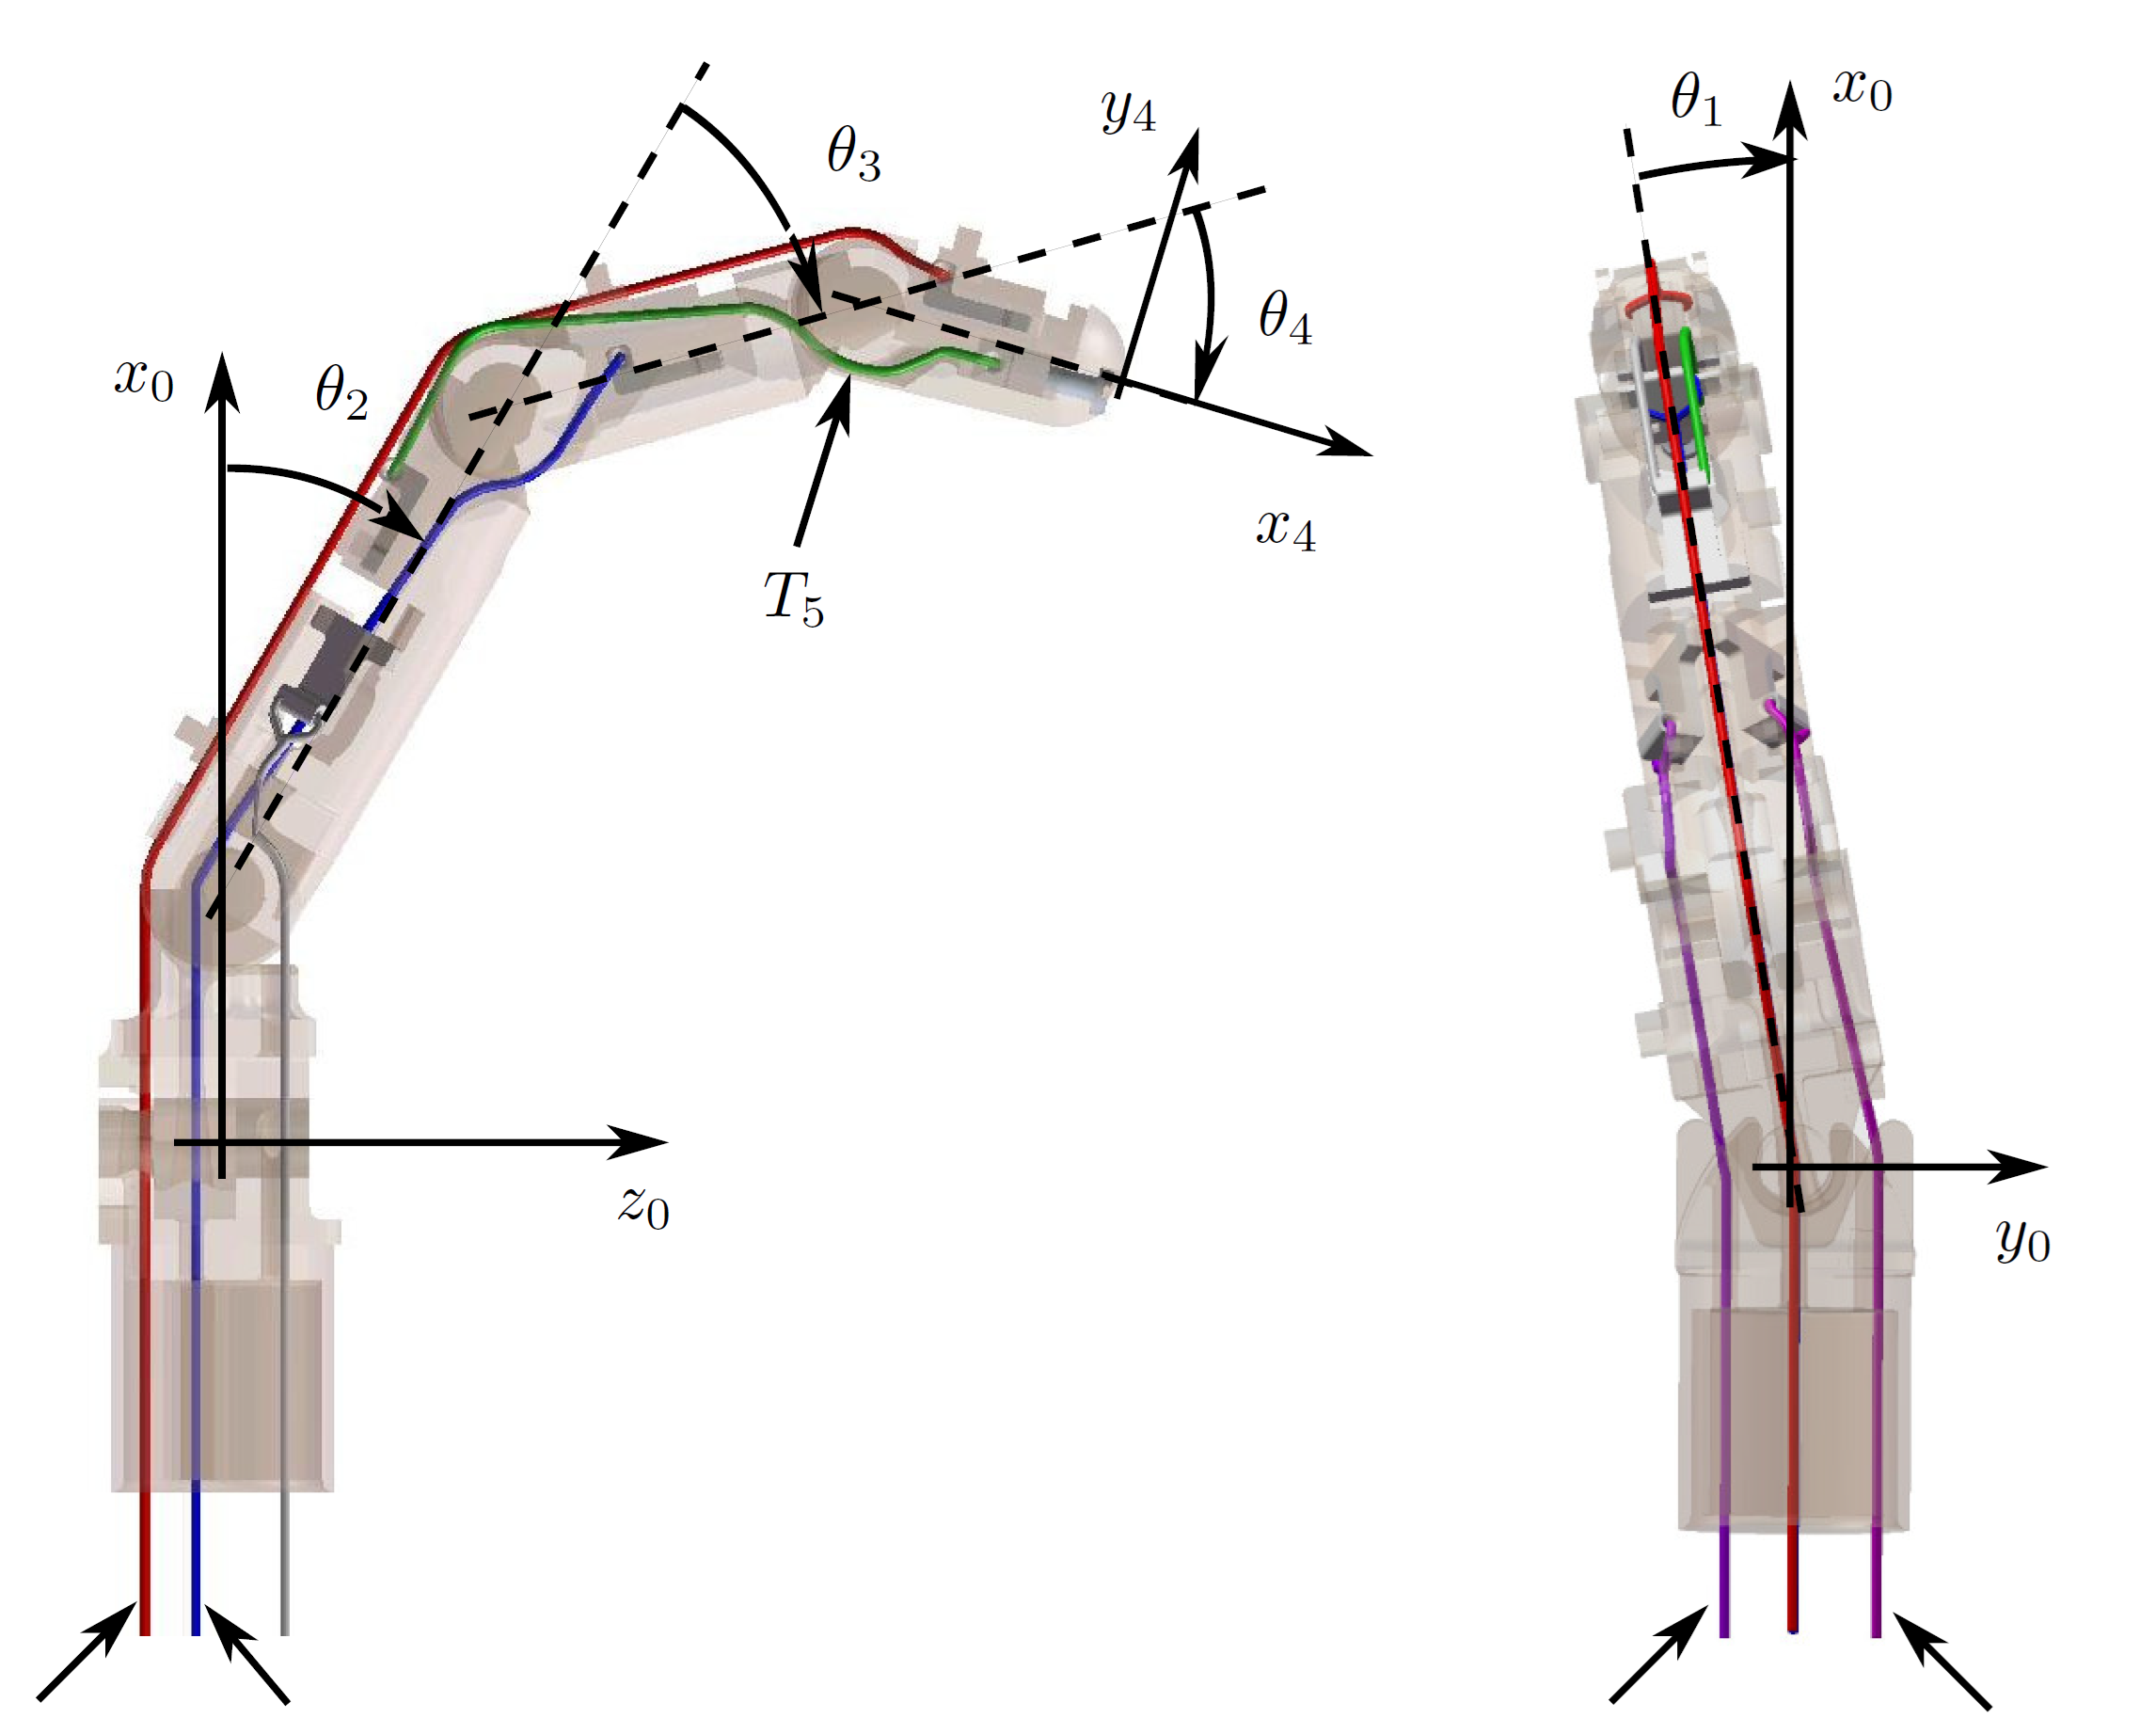
\includegraphics[width=\textwidth]{img/cover.png}
    \small (Cover image from \cite{borghesan2010design})\\
    \vspace{1.5cm} 
    \large
    \text{Thessaloniki,}\\
    \text{June 10, 2024}
    
\end{titlepage}

% Reset the fancyhdr settings for the rest of the document
\fancyhf{} % Clear all header and footer fields
\renewcommand{\headrulewidth}{0pt} % Remove the horizontal line
% Restore the original geometry
\restoregeometry
\newpage

% Table of Contents Page
\tableofcontents
\newpage

% List of tables
\listoftables
\newpage

% List of figures
\listoffigures
\newpage

% Introduction Section
\section{Introduction}
This group project is divided into four main sections: theoretical-mathematical modeling, MATLAB implementation, user interface (UI) interaction, and MQTT server for transmitting data to Team B for visualizing the equivalent of the finger in a Unity environment simulation. My contribution in this project concerns the forward and inverse kinematics, a low-level MATLAB implementation using the results of the first section I found in order for me to verify all the work I had done in the previous step, and a simple user interface creation in the MATLAB App Designer that uses the code I created in MATLAB, which helps visualize the robotic finger into an end-to-end pipeline through a UI, which paves the path for the complete UI implementation by the rest of my team. Everything I describe in the following sections is my own personal work. The diagrams and images were designed manually using Blender and ``draw.io''.


\section{Mathematical Modeling}
% Content for Mathematical Modeling
In order to comprehend, study and simulate the nature of a robotic finger and how it operates, we have first to model it, both mathematically (as equations at theoretical level) and algorithmically in a more practical way (simulation, visualization). The local reference frames and rotational axes for each joint were selected to derive the modified Denavit-Hartenberg (DH) parameters ($r_{i}$, $\alpha_{i}$, $d_i$, $\theta_i$). The modified DH parameters are more intuitive and simpler to work with, since they use the current z-axis of the joint, and there is no need for further transformations. In addition, $MCP_{aa}$ was selected as the first joint and its local frame was matched with the base frame 0, which means that upward is the z-axis and the finger extends its length along the x-axis. The next joint is $MCP_{fe}$ and then $PIP$ and $DIP$, which all three have the same rotational direction. This selection of reference frames and the order of the angles introduce only once a $\pi/2$ angle into the parameters (in addition to the normal $\theta_{i}$ angles of each joint) and simplify the subsequent equations. Figure \ref{fig:blender_axes} shows the simplified robotic finger system with reference frames, axes, lengths and angles, while Table \ref{tab:dh_parameters} shows the derived modified DH parameters.

\begin{figure}[htbp]
    \centering
    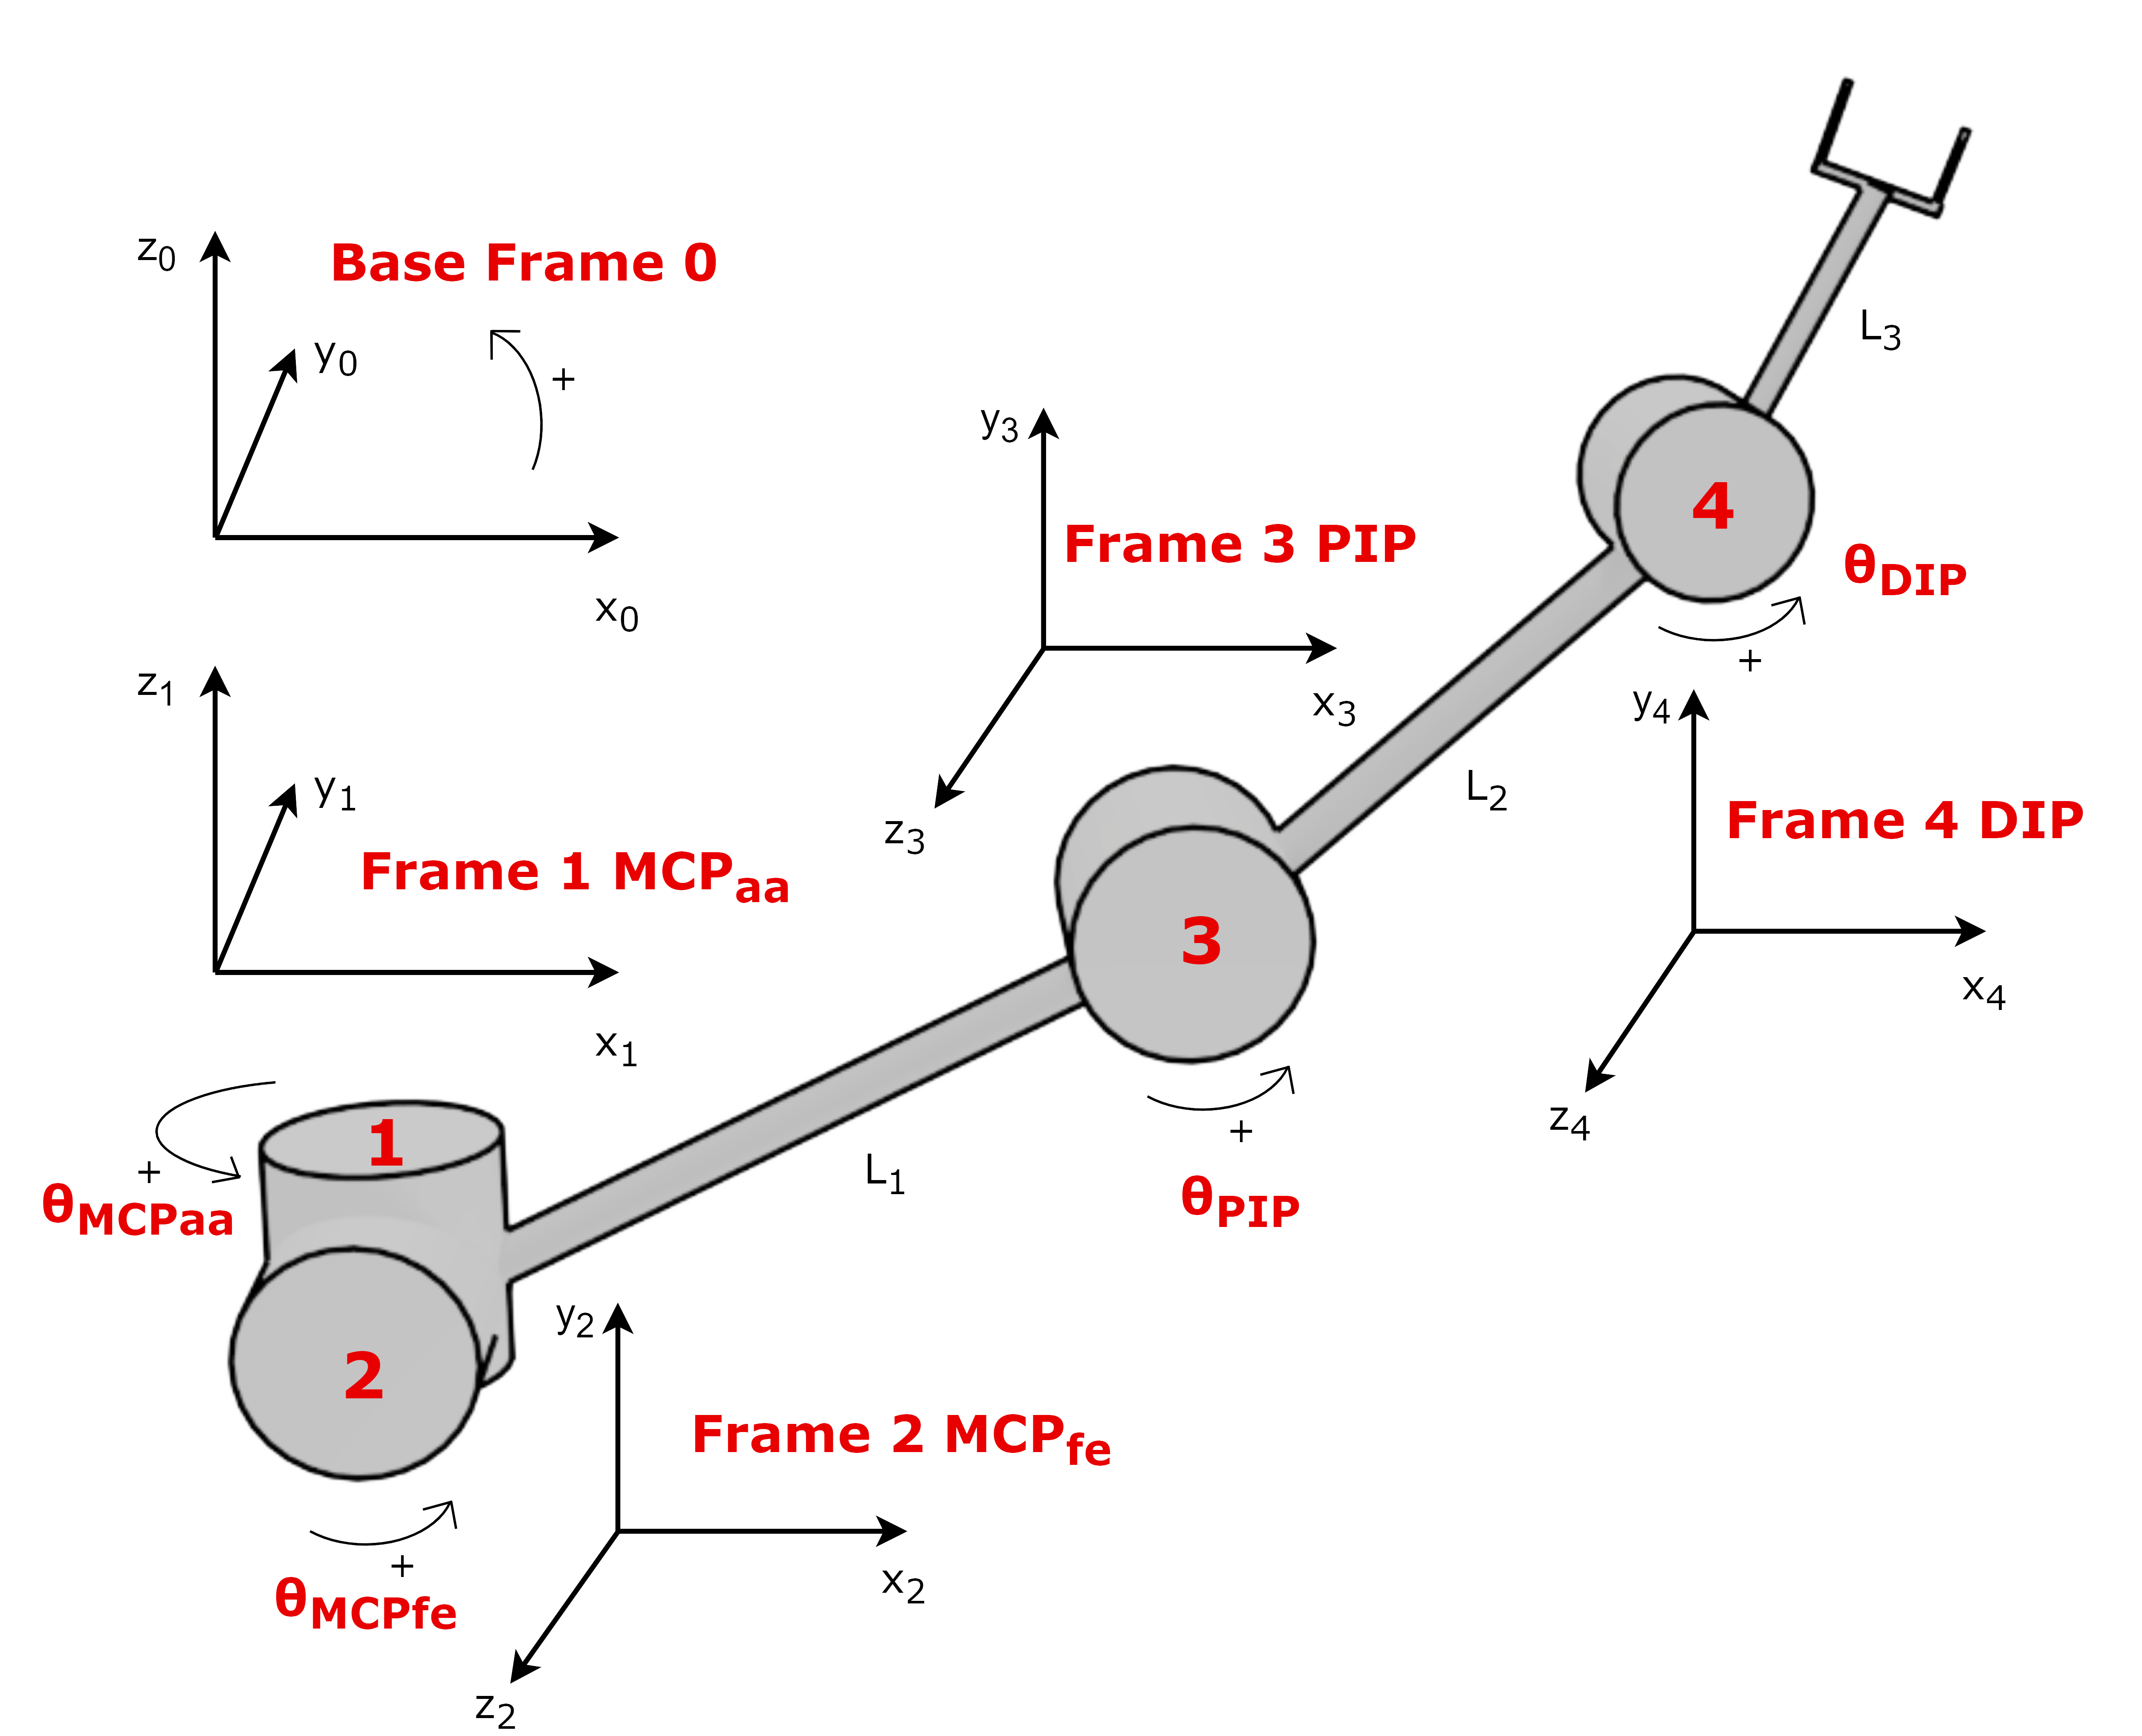
\includegraphics[width=0.88\textwidth]{img/blender_axes2.png}
    \caption{Simplified robotic finger representation with frames, designed in Blender.}
    \label{fig:blender_axes}
\end{figure}

\renewcommand{\arraystretch}{1.5} % Increase row height
\begin{table}[h]
\centering
\caption{DH Parameters Table}
\label{tab:dh_parameters}
\vspace{1pt}
\begin{tabular}{|c|c|c|c|c|}
\hline
\textit{\textbf{Joint i}} & $\boldsymbol{r_{i}}$ & $\boldsymbol{\alpha_{i}}$ & $\boldsymbol{d_i}$ & $\boldsymbol{\theta_i}$ \\ \hhline{|=|=|=|=|=|}
1 (\textit{$MCP_{aa}$}) & 0 & 0 & 0 & $\theta_{MCP_{aa}}$ \\ \hline
2 (\textit{$MCP_{fe}$}) & 0 & $\pi/2$ & 0 & $\theta_{MCP_{fe}}$ \\ \hline
3 (\textit{PIP}) & $L_1$ & 0 & 0 & $\theta_{PIP}$ \\ \hline
4 (\textit{DIP}) & $L_2$ & 0 & 0 & $\theta_{DIP}$ \\ \hline
5 (\textit{end effector}) & $L_3$ & 0 & 0 & 0 \\ \hline
\end{tabular}
\end{table}


\subsection{Forward Kinematics}
Given the lengths $L_{i}$ of the three phalanges and the angles $\theta_{i}$ of all four joints, the forward kinematics problem is to specify the final position and orientation of the end effector (fingertip) \cite{borghesan2010design, CheckValidAngles_BEST_chen2013constraint, BEST_li2022kinematic, chen2014human, tsakonas2024parameter, ueda2024development}.

The general transformation matrix between two consecutive joints is given by (\ref{eq:transformation_matrix_i}):
\begin{equation}
T_{i-1}^{i} = \left(\begin{array}{cccc}
\label{eq:transformation_matrix_i}
\cos\left(\theta \right) & -\sin\left(\theta \right) & 0 & r\\ 
\cos\left(\alpha \right)\,\sin\left(\theta \right) & \cos\left(\alpha \right)\,\cos\left(\theta \right) & -\sin\left(\alpha \right) & -d\,\sin\left(\alpha \right)\\ 
\sin\left(\alpha \right)\,\sin\left(\theta \right) & \sin\left(\alpha \right)\,\cos\left(\theta \right) & \cos\left(\alpha \right) & d\,\cos\left(\alpha \right)\\ 
0 & 0 & 0 & 1 
\end{array}\right)
\end{equation}

Applying the transformation for all four joints and for the translational end effector as well using equation (\ref{eq:transformation_matrices_product}), the final transformation matrix of the end effector is calculated (\ref{eq:transformation_matrix}) with respect to the base frame 0, which gives us the solution (equations (\ref{eq:forward_kinematics})) of the forward kinematics for the end effector (${eff}$).
\begin{equation} \label{eq:transformation_matrices_product}
    T_{0}^{eff} = T_{0}^{1} * T_{1}^{2} * T_{2}^{3} * T_{3}^{4} * T_{4}^{eff}
\end{equation}

\begin{equation}
\label{eq:transformation_matrix}
T_{0}^{eff} = \left(\begin{array}{cccc}
R_{11} & R_{12} & R_{13} & P_{14} \\
R_{21} & R_{22} & R_{23} & P_{24} \\
R_{31} & R_{32} & R_{33} & P_{34} \\
0 & 0 & 0 & 1
\end{array}\right)
\end{equation}

where:

\[
\begin{aligned}
R{11} &= \cos\left(\theta_{\mathrm{MCP_{fe}}} + \theta_{\mathrm{PIP}} + \theta_{\mathrm{DIP}}\right)\cos\left(\theta_{\mathrm{MCP_{aa}}}\right) \\
R{12} &= -\sin\left(\theta_{\mathrm{MCP_{fe}}} + \theta_{\mathrm{PIP}} + \theta_{\mathrm{DIP}}\right)\cos\left(\theta_{\mathrm{MCP_{aa}}}\right) \\
R{13} &= \sin\left(\theta_{\mathrm{MCP_{aa}}}\right) \\
P{14} &= \cos\left(\theta_{\mathrm{MCP_{aa}}}\right)\left(L_{2}\cos\left(\theta_{\mathrm{MCP_{fe}}} + \theta_{\mathrm{PIP}}\right) + L_{1}\cos\left(\theta_{\mathrm{MCP_{fe}}}\right) + L_{3}\cos\left(\theta_{\mathrm{MCP_{fe}}} + \theta_{\mathrm{PIP}} + \theta_{\mathrm{DIP}}\right)\right) \\
R{21} &= \cos\left(\theta_{\mathrm{MCP_{fe}}} + \theta_{\mathrm{PIP}} + \theta_{\mathrm{DIP}}\right)\sin\left(\theta_{\mathrm{MCP_{aa}}}\right) \\
R{22} &= -\sin\left(\theta_{\mathrm{MCP_{fe}}} + \theta_{\mathrm{PIP}} + \theta_{\mathrm{DIP}}\right)\sin\left(\theta_{\mathrm{MCP_{aa}}}\right) \\
R{23} &= -\cos\left(\theta_{\mathrm{MCP_{aa}}}\right) \\
P{24} &= \sin\left(\theta_{\mathrm{MCP_{aa}}}\right)\left(L_{2}\cos\left(\theta_{\mathrm{MCP_{fe}}} + \theta_{\mathrm{PIP}}\right) + L_{1}\cos\left(\theta_{\mathrm{MCP_{fe}}}\right) + L_{3}\cos\left(\theta_{\mathrm{MCP_{fe}}} + \theta_{\mathrm{PIP}} + \theta_{\mathrm{DIP}}\right)\right) \\
R{31} &= \sin\left(\theta_{\mathrm{MCP_{fe}}} + \theta_{\mathrm{PIP}} + \theta_{\mathrm{DIP}}\right) \\
R{32} &= \cos\left(\theta_{\mathrm{MCP_{fe}}} + \theta_{\mathrm{PIP}} + \theta_{\mathrm{DIP}}\right) \\
R{33} &= 0 \\
P{34} &= L_{2}\sin\left(\theta_{\mathrm{MCP_{fe}}} + \theta_{\mathrm{PIP}}\right) + L_{1}\sin\left(\theta_{\mathrm{MCP_{fe}}}\right) + L_{3}\sin\left(\theta_{\mathrm{MCP_{fe}}} + \theta_{\mathrm{PIP}} + \theta_{\mathrm{DIP}}\right)
\end{aligned}
\]

\begin{equation}
\label{eq:forward_kinematics}
\begin{aligned}
    x_{eff} & = P{14}\\
    y_{eff} & = P{24}\\
    z_{eff} & = P{34}
\end{aligned}
\end{equation}

A challenge I faced during forward kinematics was to understand the DH parameters and how the reference frames should be set and what values should be assigned as parameters, which is the first but crucial step in the methodology of robotics. Also, the proper selection of reference frames is very important as a convention, because it affects the simplicity of the derived equations after the transformation matrices calculations.


\subsection{Inverse Kinematics}
On the contrary, given the end position of the fingertip and its orientation, the inverse kinematics problem seeks to find all four angles that correspond to that end state (position and orientation). Solving the inverse kinematics problem in closed-form algebraic equations is often a difficult task, especially if the joints are too many or the system architecture is complex. Usually, computational numeric methods are applied iteratively to approximate the solutions for the angles. Apart from numeric approaches, there are two ways to solve the inverse problem in closed form equations, either algebraically or geometrically \cite{craig2009introduction, CheckValidAngles_BEST_chen2013constraint, BEST_li2022kinematic, chavdarov2022algorithm, nunez2015design}. I opted for the geometric approach, which helps visualize the system comprehensively and perhaps find the solution in a simpler way. The following diagrams in Figure \ref{fig:finger_all_inverse} show the top-view (x-y) and the side-view (x-z) planes of the finger, always with respect to the base frame of reference, which means that the local rotational z-axes for the last three joints ($MCP_{fe}, PIP, DIP$) are aligned with the $-y$ axis of the base frame 0. To visualize in space all this system configuration and write down equations describing each joint, equations originating from geometrical analysis, was quite challenging and fascinating, since a clear and comprehensive diagram depicting everything is of utmost importance. Also, apart from the end position, the end orientation of the fingertip is required, which here translates to the cumulative angle on the x-z plane with respect to the x-axis of the base frame 0. This angle, let's denote it as $\epsilon$, is equal to:\\
\begin{equation}
    \epsilon = \epsilon_{234} = \theta_{MCP_{fe}} + \theta_{PIP} + \theta_{DIP}
\end{equation}

\begin{figure}[htbp]
    \centering
    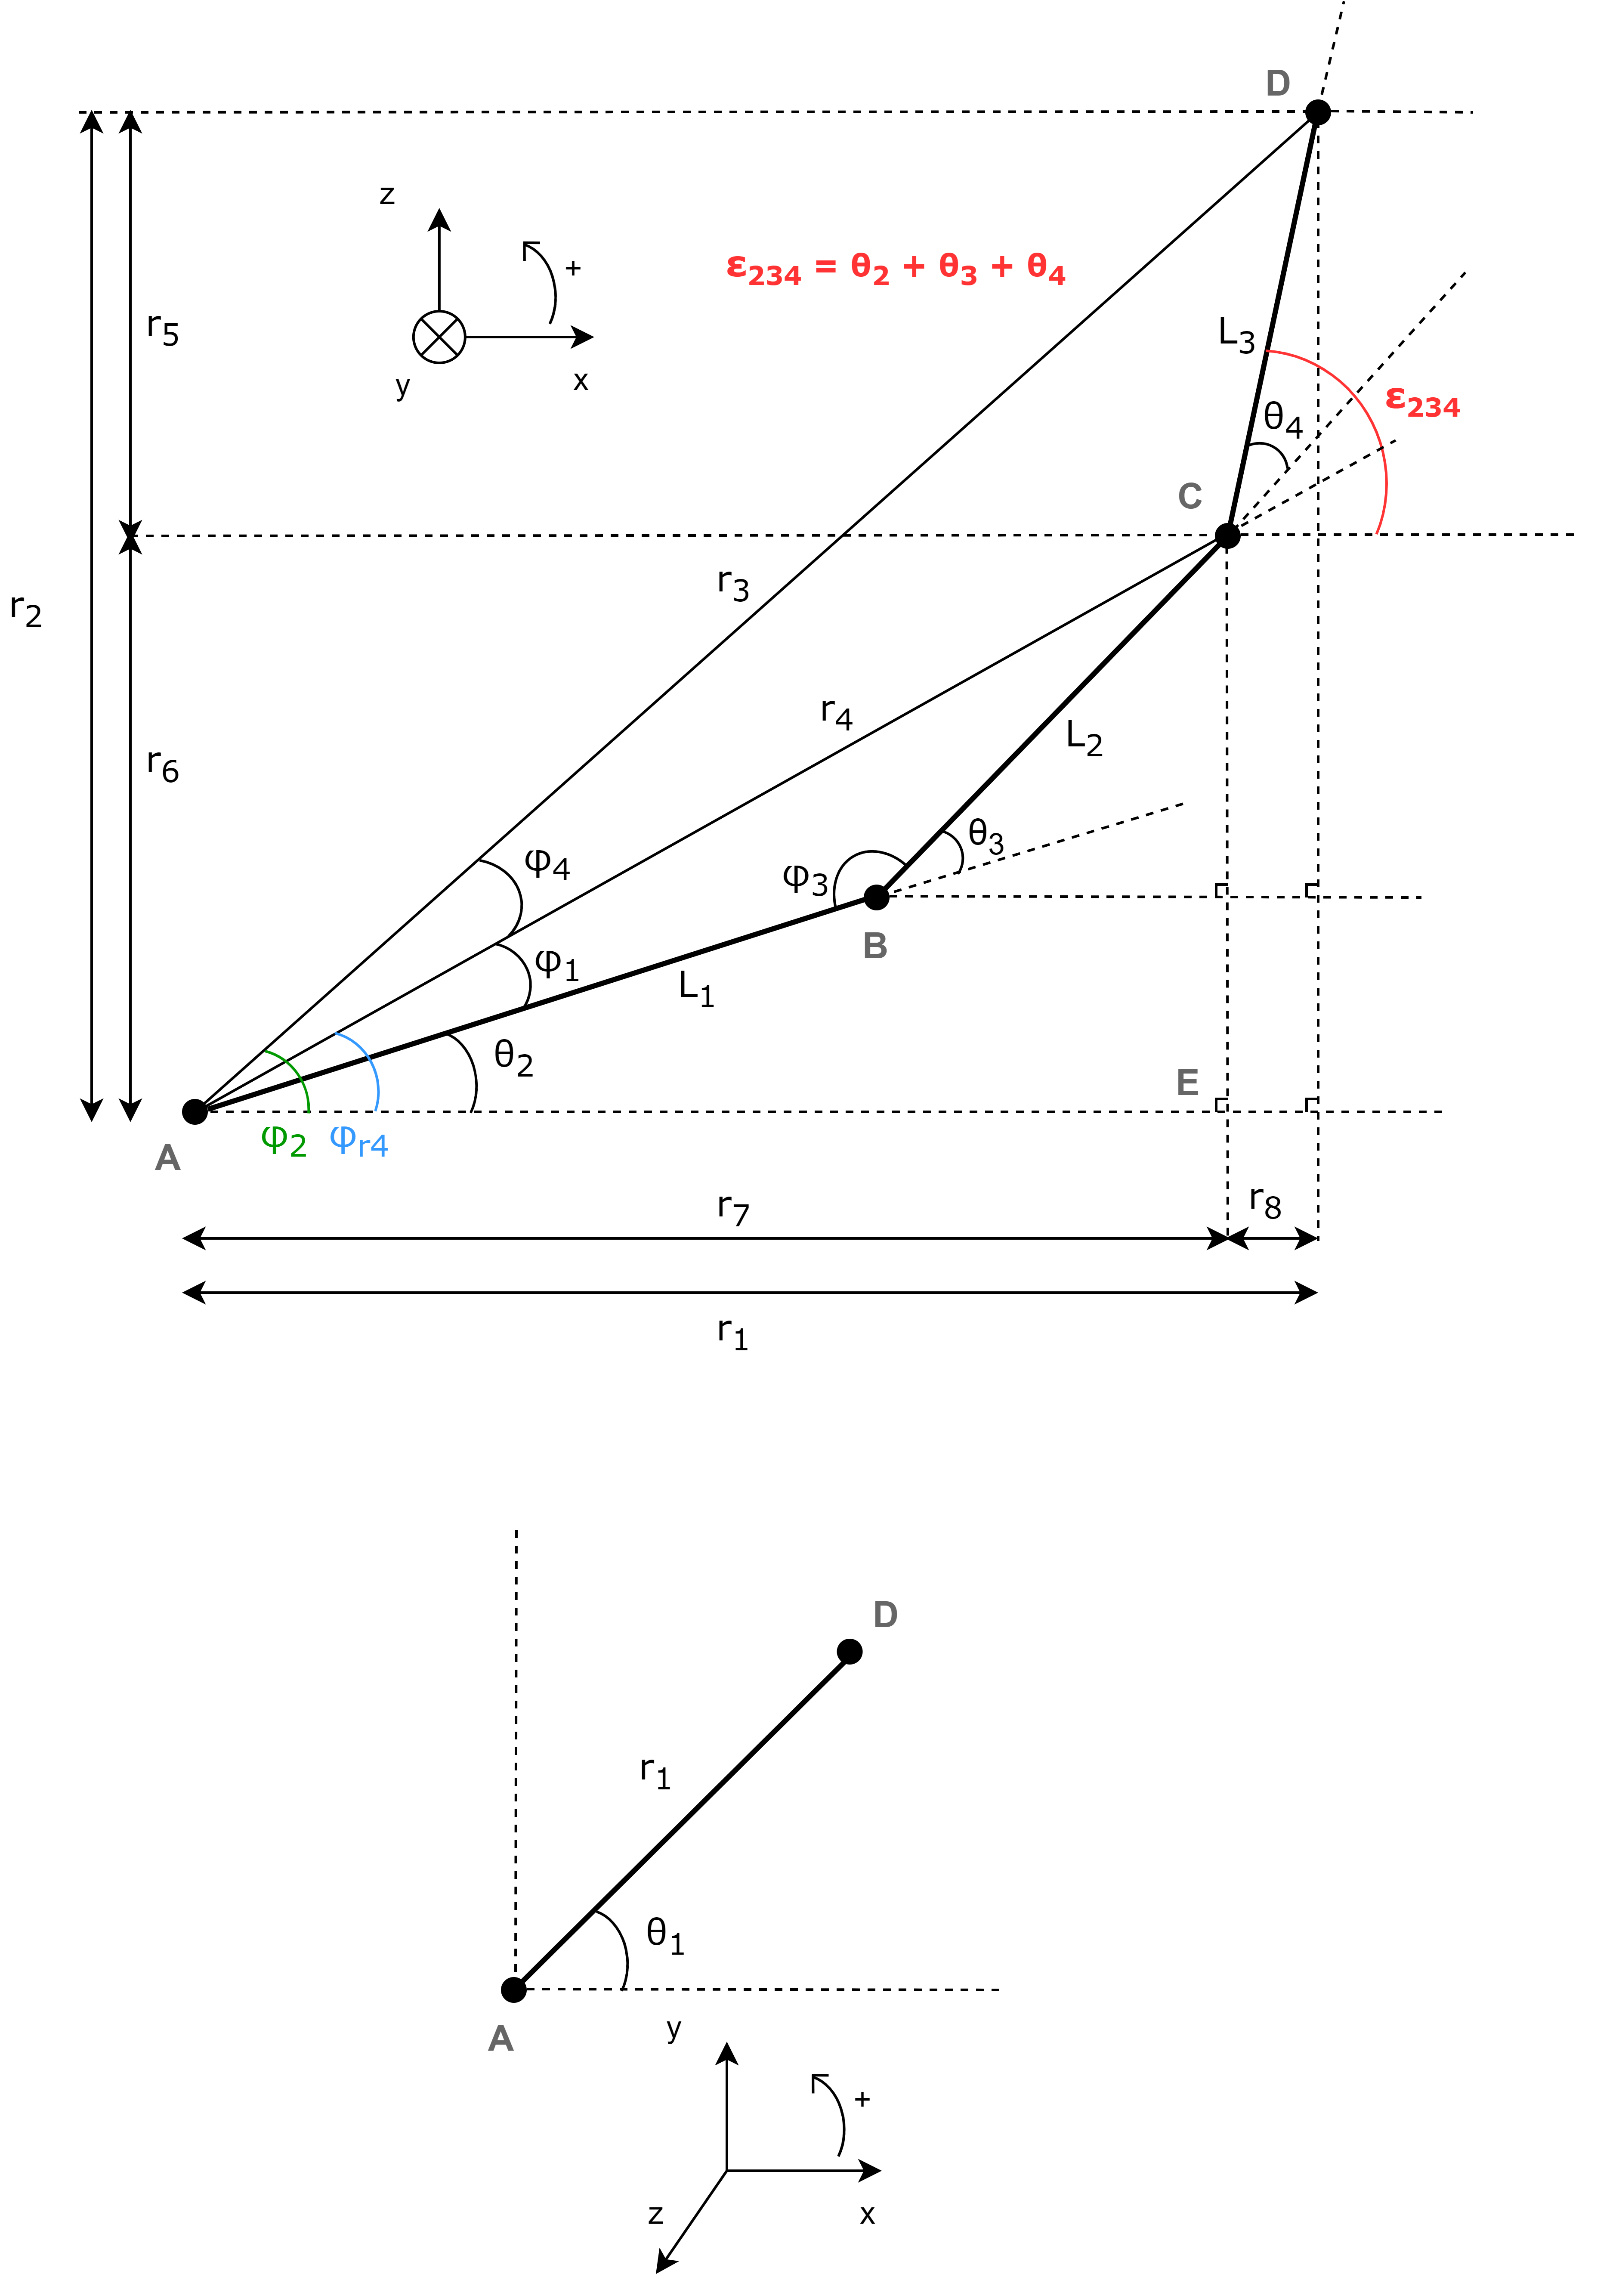
\includegraphics[width=1\textwidth]{img/finger_diagram_all.png}
    \caption{Extensive top-view (x-y plane) and side-view (x-z plane) depiction of the robotic finger, designed in ``draw.io'', for solving the inverse kinematics problem with geometric approach.}
    \label{fig:finger_all_inverse}
\end{figure}

Therefore, given the $x, y, z$ and the angle $\epsilon$, the inverse kinematics problem must be solved. In order for the equations to be more concise, the following notation will be used:\\
\begin{equation}
\label{eq:given}
\begin{aligned}
    x & = x_{eff} &\text{ (given)}\\
    y & = y_{eff} &\text{ (given)}\\
    z & = z_{eff} &\text{ (given)}\\
    \theta_{1} & = \theta_{MCP_{aa}}\\
    \theta_{2} & = \theta_{MCP_{fe}}\\
    \theta_{3} & = \theta_{PIP}\\
    \theta_{4} & = \theta_{DIP}\\
    \theta_{234} & = \theta_{2} + \theta_{3} + \theta_{4} = \epsilon &\text{ (given)}
\end{aligned}
\end{equation}

Starting from the top-view diagram, for the triangle formed by $r_{1}$, $x$ and $y$:\\
\begin{equation}
\label{eq:theta1Sol}
    \tan(\theta_{1}) = \frac{y}{x} \implies \boxed{\theta_{1} = \arctan\left(\frac{y}{x}\right)}
\end{equation}
\begin{equation}
    r_{1} = \sqrt{x^{2} + y^{2}}
\end{equation}

Moving on to the side-view diagram, the following equations apply:\\
\begin{equation}
\begin{aligned}
    \phi_{2} & = \phi_{1} + \phi_{4} + \theta_{2}\\
    r_{2} & = z
\end{aligned}
\end{equation}
\begin{equation}
    r_{3}  = \sqrt{r_{1}^{2} + r_{2}^{2}} \implies r_{3} = \sqrt{x^{2} + y^{2} + z^{2}}
\end{equation}
\begin{equation}
    \tan(\phi_{2}) = \frac{r_{2}}{r_{1}} \implies \phi_{2} = \arctan\left(\frac{z}{\sqrt{x^{2} + y^{2}}}\right)
\end{equation}

\begin{equation}
\begin{aligned}
    r_{5} & = L_{3}\sin(\epsilon)\\
    r_{6} & = r_{2} - r_{5}\\
    r_{8} & = L_{3}\cos(\epsilon)\\    
    r_{7} & = r_{1} - r_{8}
\end{aligned}
\end{equation}
\begin{equation}
     \tan(\phi_{r_{4}}) = \frac{r_{6}}{r_{7}} \implies \phi_{r_{4}} = \arctan\left(\frac{z - L_{3}\cdot\sin(\epsilon)}{\sqrt{x^{2} + y^{2}} - L_{3}\cdot\cos(\epsilon)}\right)
\end{equation}

Applying the cosine rule in the triangle $\overset{\triangle}{ABC}$ and using the properties of $\overset{\triangle}{AEC}$:\\
\begin{equation}
\label{eq:phi1}
    L_{2}^{2} = L_{1}^{2} + r_{4}^{2} - 2L_{1}r_{4}\cdot\cos(\phi_{1})
\end{equation}
\begin{equation}
\label{eq:abc_r4}
    r_{4}^{2} = L_{1}^{2} + L_{2}^{2} - 2L_{1}L_{2}\cdot\cos(\phi_{3}) \overset{\phi_{3} = \pi - \theta_{3}}{\implies} r_{4}^{2} = L_{1}^{2} + L_{2}^{2} + 2L_{1}L_{2}\cdot\cos(\theta_{3})
\end{equation}

\begin{equation}
\label{eq:r4}
\begin{aligned}
     r_{4}^{2} & = r_{7}^{2} + r_{6}^{2} = (r_{1} - r_{8})^{2} + (r_{2} - r_{5})^{2} \\
     \implies r_{4}^{2} & = x^{2} + y^{2} + z^{2} + L_{3}^{2} - 2L_{3}(\sqrt{x^{2} + y^{2}}\cdot\cos(\epsilon) + z\cdot\sin(\epsilon))
\end{aligned}
\end{equation}

Using the above equation (\ref{eq:r4}), we can now solve for $\theta_{3}$ in equation (\ref{eq:abc_r4}):
\begin{equation}
\label{eq:theta3Sol}
     \boxed{\theta_{3} = \arccos\left(\frac{x^{2} + y^{2} + z^{2} + L_{3}^{2} - L_{1}^{2} - L_{2}^{2} - 2L_{3}(\sqrt{x^{2} + y^{2}}\cdot\cos(\epsilon) + z\cdot\sin(\epsilon))}{2L_{1}L_{2}}\right)}
\end{equation}

\begin{equation}
\label{eq:phi4}
     \phi_{4} = \phi_{2} - \phi_{r_{4}} = \arctan\left(\frac{z}{\sqrt{x^{2} + y^{2}}}\right) - \arctan\left(\frac{z - L_{3}\cdot\sin(\epsilon)}{\sqrt{x^{2} + y^{2}} - L_{3}\cdot\cos(\epsilon)}\right)
\end{equation}

From equation (\ref{eq:phi1}) we can now solve for $\phi_{1}$, using equation (\ref{eq:r4}):
\begin{equation}
\label{eq:phi1Sol}
     \phi_{1} = \arccos\left(\frac{x^{2} + y^{2} + z^{2} + L_{1}^{2} + L_{3}^{2} - L_{2}^{2} - 2L_{3}(\sqrt{x^{2} + y^{2}}\cdot\cos(\epsilon) + z\cdot\sin(\epsilon))}{2L_{1}\sqrt{x^{2} + y^{2} + z^{2} + L_{3}^{2} - 2L_{3}(\sqrt{x^{2} + y^{2}}\cdot\cos(\epsilon) + z\cdot\sin(\epsilon))}}\right)
\end{equation}

From equations (\ref{eq:phi4}) and (\ref{eq:phi1Sol}), we can now solve for $\theta_{2}$:
\begin{equation}
    \theta_{2} = \phi_{2} - \phi_{1} - \phi_{4}
\end{equation}
\begin{equation}
\label{eq:theta2Sol}
\boxed{
\begin{aligned}
     \implies\theta_{2} & = \arctan\left(\frac{z - L_{3}\cdot\sin(\epsilon)}{\sqrt{x^{2} + y^{2}} - L_{3}\cdot\cos(\epsilon)}\right) \\
     &- \arccos\left(\frac{x^{2} + y^{2} + z^{2} + L_{1}^{2} + L_{3}^{2} - L_{2}^{2} - 2L_{3}(\sqrt{x^{2} + y^{2}}\cdot\cos(\epsilon) + z\cdot\sin(\epsilon))}{2L_{1}\sqrt{x^{2} + y^{2} + z^{2} + L_{3}^{2} - 2L_{3}(\sqrt{x^{2} + y^{2}}\cdot\cos(\epsilon) + z\cdot\sin(\epsilon))}}\right)
\end{aligned}
}
\end{equation}

Finally, after having calculated $\theta_{2}$ and $\theta_{3}$ in equations (\ref{eq:theta2Sol}) and (\ref{eq:theta3Sol}) respectively, and since we know $\epsilon$ (given), we can now also solve for $\theta_{4}$, which will be the last angle to be calculated.
\begin{equation}
\label{eq:theta4Sol}
     \boxed{\theta_{4} = \epsilon - \theta_{2} - \theta_{3}}
\end{equation}


\section{MATLAB Code Implementation}
To verify all the above, I deemed it prudent to develop MATLAB scripts and functions that implement such example states of the robot finger, mostly the inverse kinematics followed by a confirmatory forward kinematics. All the relative MATLAB code files have been uploaded in my personal \href{https://github.com/Inglezos/BME_Robotic_Finger_Project}{Github} repository, along with detailed code documentation and comments. Essentially, I have incorporated the transformation matrices equations and the inverse kinematics angles equations into the code for solving both forward and inverse kinematics problem as low-level implementation (while on the contrary, a high-level implementation would use Simulink-Simscape or even ROS).\\

For example, ``forward\_kinematics.mlx'' script calculates the end-effector's position and orientation for given joint angles and conversely, ``inverse\_kinematics\_equations.mlx'' script determines the joint angles needed for a desired end-effector state (position and orientation-angle). Literature suggests \cite{CheckValidAngles_BEST_chen2013constraint, CheckValidAngles_cobos2008efficient, CheckValidAngles_lee2014flexion, CheckValidAngles_ngeo2014continuous} that there are some specific angle ranges for each joint per finger that are considered as valid and are widely accepted, therefore a validity check shall be included for the angles found during inverse solution. Keeping the minimum and maximum values across all fingers (we did not specify a finger but rather we have considered the general case of ``index, middle, ring, little'' fingers, except for thumb. As future work, the valid range could be further narrowed down for a specific finger, or even include the thumb as well. These constraints are imposed on the angles using ``check\_valid\_angles.m''. The ranges used are shown in Table \ref{tab:valid_angles}.

\begin{table}[htbp]
\centering
\caption{Generalized valid angle ranges for joints.}
\label{tab:valid_angles}
\vspace{1pt}
\begin{tabular}{|c|c|c|c|c|}
\hline
\textit{\textbf{Degrees}} & $\boldsymbol{\theta_{MCP_{aa}}}$ & $\boldsymbol{\theta_{MCP_{fe}}}$ & $\boldsymbol{\theta_{PIP}}$ & $\boldsymbol{\theta_{DIP}}$ \\ \hhline{|=|=|=|=|=|}
Min & -60 & -55 & -27.5 & -31\\ \hline
Max & +60 & +90 & +135 & +97.5\\ \hline
\end{tabular}
\end{table}


\section{Graphical User Interface (GUI) Development}
Finally, I created a simple but effective graphical user interface environment to test the above end-to-end pipeline of desired fingertip position, inverse kinematics calculations and angles derivation. The relevant GUI files I created are ``GUI\_forward\_kinematics.m'' (calculates forward kinematics for given angles), ``GUI\_inverse\_kinematics.m'' (solves inverse kinematics for a user-specified end position and orientation) and ``GUI\_get\_all\_positions.m'' (returns the positions for the three joints plus for end effector for explicit visualization inside the GUI). The returned angles are validated using ``check\_valid\_angles()'' and in case the end position is not valid (due to the limited phalanges lengths or due to out-of-range angles), a proper error pop-up message is displayed to the user.\\

The user interface is intuitive with a simplified 3D representation of the finger (joints and phalanges). The user can set values for the lengths of each phalange ($L_{1}, L_{2}, L_{3}$) and can specify the desired end state of the fingertip (position $x, y, z$ and angle $\epsilon$) through dedicated text fields and sliders. The complete code for my GUI version is the ``Robotic\_Finger\_GUI\_App.mlapp'' file. The app design was challenging, as I had no prior experience with GUI development. My GUI work lays the foundation for an extensive GUI version with even more features and functionalities. The Figures \ref{fig:GUI_full} and \ref{fig:GUI_error} show an example of my GUI implementation. The calculated values for the inverse kinematics for all four angles are displayed in the ``Theta Values'' field. These values afterwards can be transmitted to the Team B via the MQTT server.

\begin{figure}[htbp]
    \centering
    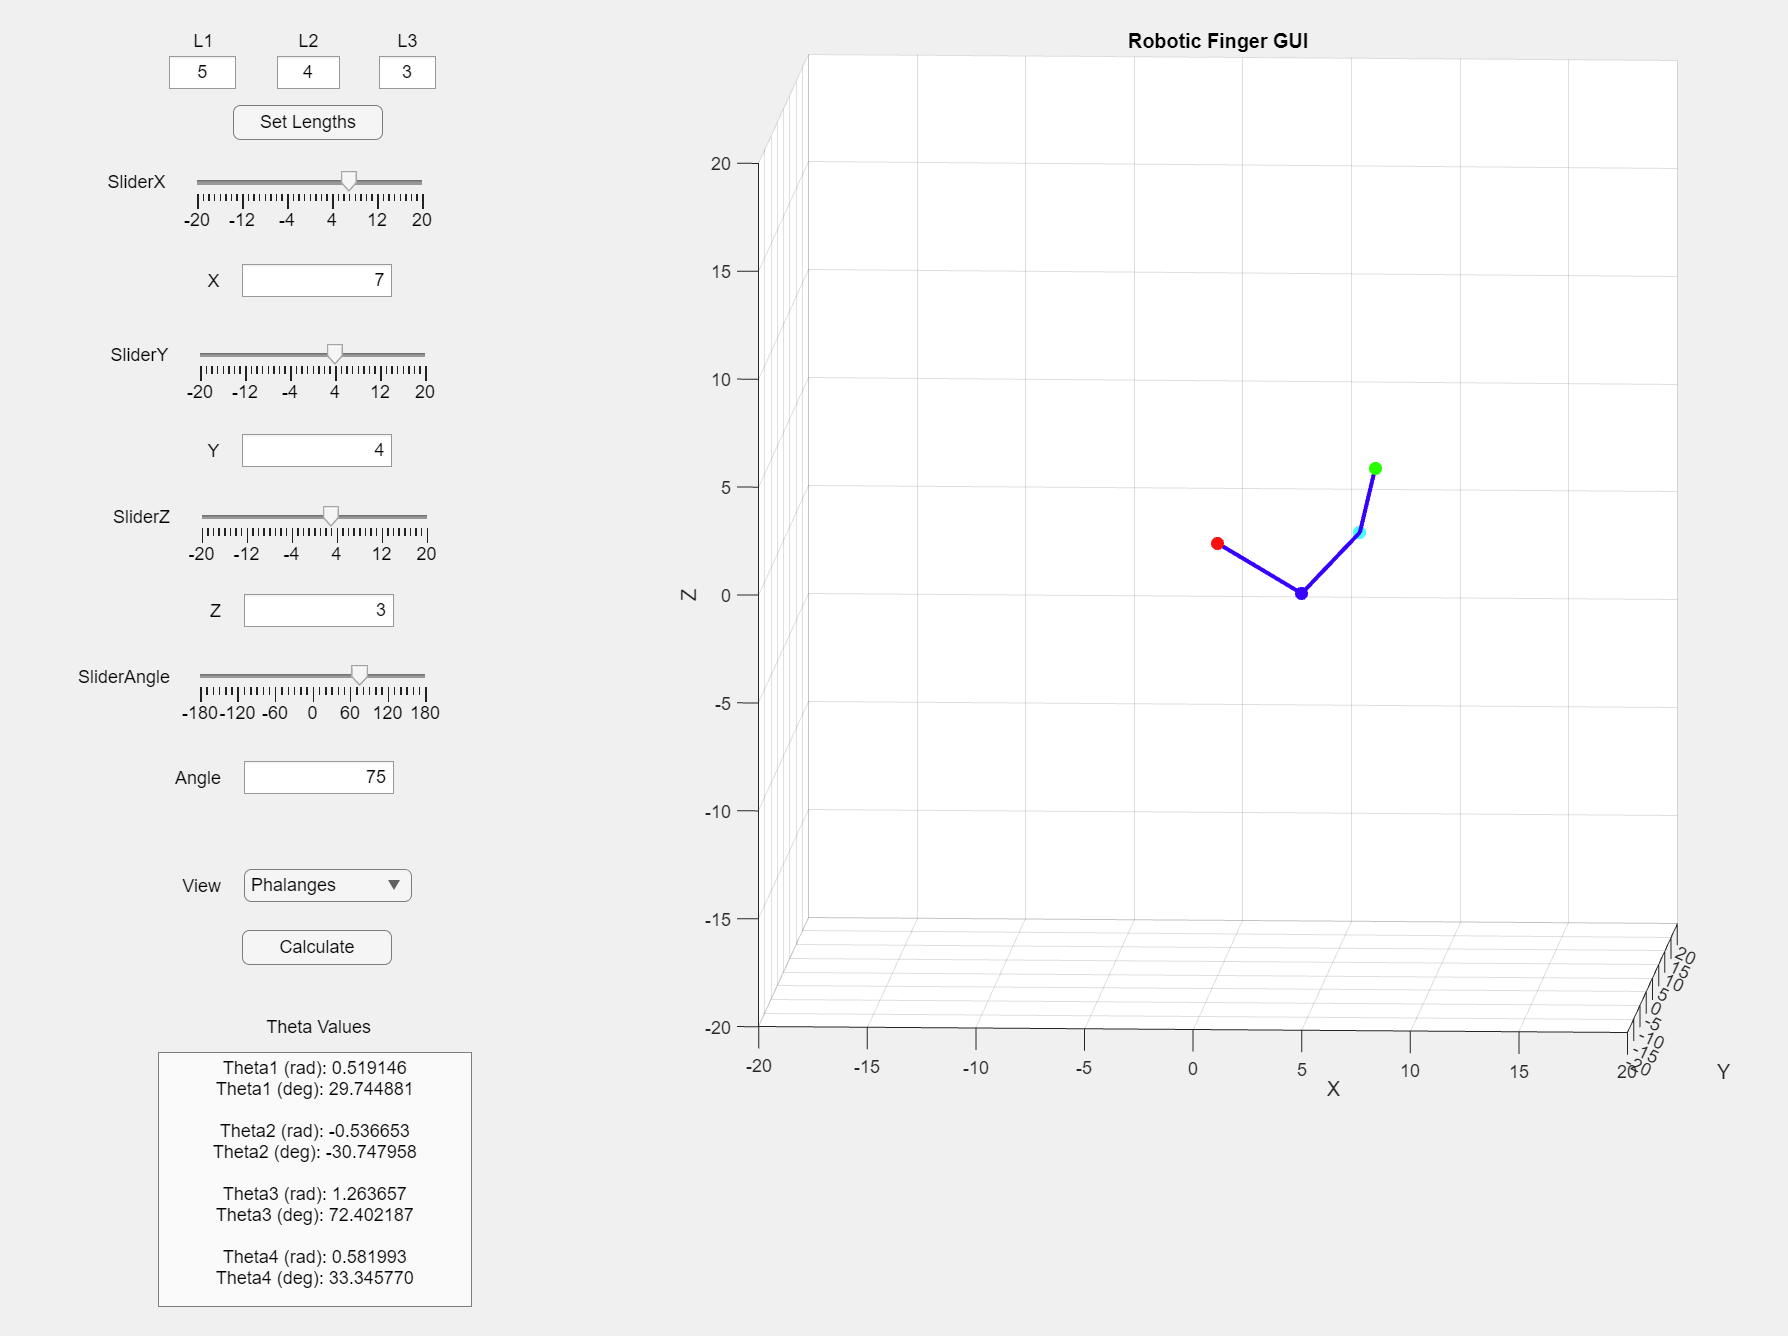
\includegraphics[width=1\textwidth]{img/GUI_full.png}
    \caption{An intuitive user interface environment for controlling the robotic finger. On the left, through the configuration fields and sliders, the user can set the length of each phalange, and manipulate the end position in 3D space (x, y, z) and the end orientation (angle). On the right, the finger's visualization of the user-specified end position is shown.}
    \label{fig:GUI_full}
\end{figure}

\begin{figure}[htbp]
    \centering
    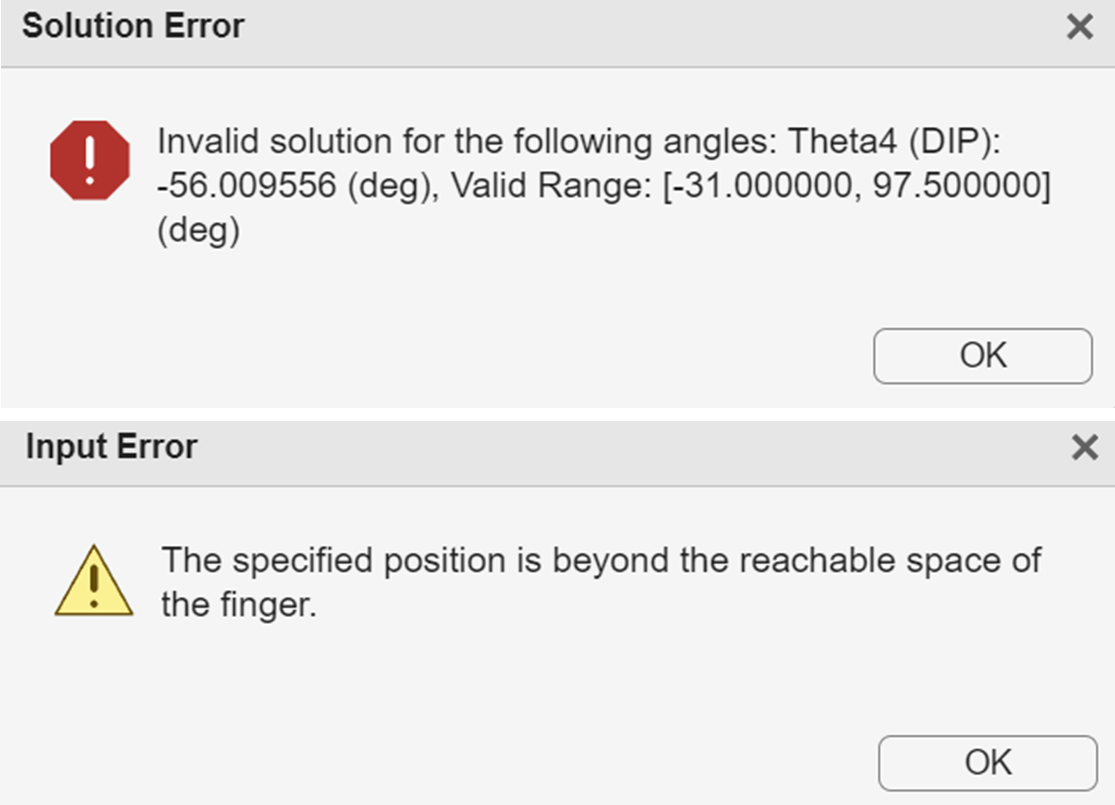
\includegraphics[width=0.75\textwidth]{img/GUI_error.png}
    \caption{GUI error messages in case the user has specified an invalid end position.}
    \label{fig:GUI_error}
\end{figure}


\section{Conclusion}
In this personal report, I have described in detail my contributions to three aspects of the project, to the mathematical modeling from scratch, to a low-level MATLAB code implementation, and to the creation of a preliminary graphical user interface environment for manipulating the robotic finger. All this leads to the implementation of an effective, comprehensive, and user-intuitive system with a solid theoretical background and technical analysis, while further refinements and additional functionalities can be explored more systematically as future work.\\

\newpage

% \section{References}
% Add References to the table of contents
\addcontentsline{toc}{section}{References}
\nocite{*}
\bibliographystyle{IEEEtran}
\bibliography{references}

\end{document}